\documentclass[10pt,twocolumn]{article}
\usepackage[letterpaper,margin=1in]{geometry}
\usepackage{times,amsmath,amssymb,graphicx,booktabs,cite,hyperref,xcolor,url}
\setlength{\columnsep}{0.6cm}
\title{\bf DocScout: When Does Read-Budget Reinforcement Learning\\
Help for Document-Search Agents?\\
\normalsize A Diagnose-Fix-Verify Study: When (and Why) Read-Budget RL Pays Off}
\author{Anonymous (AAAI submission, under review)}
\date{}

\newcommand{\eff}{\mathrm{eff}}

\begin{document}
\twocolumn[
\maketitle
\begin{abstract}
A retrieval agent that decides \emph{how much to read} and \emph{when to stop} should beat fixed top-$k$ RAG: matching its accuracy while spending fewer tokens on irrelevant text. We test this for natural-language documents. \textbf{DocScout} is a tool-using agent (\texttt{search}/\texttt{read}/\texttt{expand}/\texttt{answer}) trained with a read-budget reward, in the spirit of CodeScout but with read-cost as a first-class objective. Our first design was silently inert: REINFORCE produced \emph{zero} policy movement (0/150 held-out instances changed), and the agent was dominated by one-shot RAG. Rather than tune until it won, a diagnose-before-train protocol traced this to two fixable design flaws: (i) the reward was \emph{flat at the SFT optimum} (a weak efficiency term the SFT already maximized), and (ii) the learning rate was too small to move a peaked-SFT policy. Fixing both---a reward with a term the SFT does \emph{not} maximize (a per-read action cost, which creates gradient variance) plus a selection bonus (rewarding reading the gold section first), at an adequate LR---yields a strong \emph{positive} result: read-budget RL \textbf{Pareto-dominates} both SFT and one-shot RAG on the accuracy-per-read-token frontier, reaching \textbf{0.84 accuracy at 170 committed read-tokens} (reading exactly one section) vs.\ SFT's 0.65 and RAG-$k$1's 0.753@182, and matching RAG-$k$5's accuracy at \textbf{18.7\%} of its read cost (5.3$\times$ fewer tokens). The gain is consistent across two seeds and decomposes cleanly: RL fixes selection (gold-hit 84\% with one read, $>$ RAG's 75\%), extraction (accuracy given gold read: 0.72$\to$1.0), and efficiency (reads per question: 3.25$\to$1.0). We contribute (a) the positive frontier result, (b) the diagnose-fix-verify methodology that turned an inert setup into a working one, and (c) a mechanistic recipe (non-flat reward + adequate LR) for read-budget RL on peaked-SFT tool agents.
\end{abstract}
\vspace{1em}
]

\section{Introduction}
\label{sec:intro}

Standard retrieval-augmented generation (RAG)~\cite{rag2020} retrieves a fixed number of passages once and pastes them into the prompt. This is wasteful---irrelevant passages consume context---and gives the model no control over \emph{how much} it reads. A natural fix is an \emph{agent} that can call \texttt{search}, selectively \texttt{read} full sections, and \texttt{answer} when it has enough evidence, trained with reinforcement learning (RL) to optimize not just accuracy but \emph{reading efficiency}. This is the premise of recent tool-using retrieval agents~\cite{searchr1,research,autosearch} and of CodeScout~\cite{codescout2026}, which trains a code-localization agent with RL and a minimal tool set.

We ask the natural-language analogue: \textbf{can a read-budget RL agent dominate fixed-$k$ RAG on the accuracy-per-read-token frontier?} We build DocScout, port CodeScout's minimal-tool recipe to text documents, and make read-budget a first-class reward objective via an \emph{efficiency-ratio} term (the fraction of read tokens that are gold evidence).

\textbf{Our first design was silently inert---and we report the fix, not the burial.} With a natural read-budget reward (efficiency-ratio), REINFORCE produced \emph{zero} policy movement (0/150 held-out instances changed), leaving the agent dominated by one-shot RAG. We did not tune until the method won; we diagnosed the failure, fixed it, and verified the fix:

\begin{itemize}\itemsep0pt
\item \textbf{Diagnose.} The reward was \emph{flat at the SFT optimum}: SFT demonstrations already read the gold section, so the efficiency-ratio was already $\approx$1 and the reward could not distinguish better policies. Worse, the learning rate ($10^{-6}$) was too small for a LoRA update to change the peaked-SFT greedy decode at all.
\item \textbf{Fix.} Add a reward term the SFT does \emph{not} maximize---a per-read \emph{action cost} that penalizes the over-reading SFT inherits, creating real gradient variance---plus a \emph{selection bonus} that rewards reading the gold section first, and raise the LR to $10^{-5}$.
\item \textbf{Verify.} The fixed read-budget RL now \emph{Pareto-dominates} SFT and one-shot RAG: 0.84 accuracy at 170 committed read-tokens (reading exactly one section) vs.\ SFT's 0.65 and RAG-$k$1's 0.753@182, matching RAG-$k$5's accuracy at 18.7\% of its read cost.
\end{itemize}

\paragraph{Contributions.}
\begin{itemize}\itemsep0pt
\item A \textbf{positive frontier result}: read-budget RL Pareto-dominates SFT and fixed-$k$ RAG on the accuracy-per-read-token frontier (0.84@170 BPE, $n_{\text{read}}{=}1$, consistent over 2 seeds and 6 checkpoints; \S\ref{sec:results}).
\item A \textbf{mechanistic recipe} for read-budget RL on peaked-SFT tool agents: the reward must contain a term the SFT does \emph{not} maximize (action cost $\Rightarrow$ gradient variance) plus a selection objective, at an LR that can move the greedy policy (\S\ref{sec:analysis}).
\item A \textbf{diagnose-fix-verify methodology} that turned an inert setup into a working one, and that independently surfaced three integrity bugs in our own earlier results (App.~\ref{app:audit})---a low-cost guardrail for agentic-RL work.
\item A \textbf{realistic-scale, leakage-free substrate} (synth-v3) and an honest BPE-token cost metric, where RAG genuinely desaturates (\S\ref{sec:data}).
\item Two \textbf{reusable findings}: the SFT stop-failure pathology and its $4\times$ answer-up-weighting fix, and REINFORCE-with-baseline's superiority over GRPO on peaked-SFT tool agents (\S\ref{sec:setup}).
\end{itemize}

\paragraph{Why the journey matters.} Reporting only the final positive result would hide the trap: a read-budget reward that \emph{looks} reasonable is silently inert on a peaked-SFT policy, and an LR that is standard for full fine-tuning is too small for LoRA RL. By exposing the inert v1 and its fix, we make it cheaper for others to get read-budget RL to work---and harder to mistake ``RL didn't help'' for ``RL can't help.''

\section{Related Work}
\label{sec:related}
\textbf{Tool-using retrieval agents.} ReAct~\cite{react2023} and WebGPT~\cite{webgpt2022} establish tool-using agents for QA but do not shape read cost with RL. FLARE~\cite{flare} retrieves actively when generation confidence drops---a prompting-time heuristic for ``when to retrieve,'' orthogonal to our learned, reward-shaped reading depth. Search-R1~\cite{searchr1}, ReSearch~\cite{research}, AutoSearch~\cite{autosearch} and dynamic-depth variants~\cite{dynsearchr1} train retrieval agents with RL, but they optimize answer accuracy and search \emph{depth on the open web} (how many searches), not \emph{intra-document reading volume} against a fixed corpus with section-locatable evidence. Their cost axis is \#queries; ours is committed read tokens.

\textbf{CodeScout and the minimal-tool recipe.} CodeScout~\cite{codescout2026} is the closest analogue: a minimal-tool RL agent for code localization. Two key transfers guided our design: (i) a minimal tool set keeps the action space small and rollouts cheap (no execution/sandbox needed for localization, just as none is needed for reading); (ii) CodeScout reports an efficiency \emph{evaluation} (steps/tokens, their Tab.~6) but its training reward contains \emph{no} efficiency term---efficiency is enforced only by a hard \texttt{max\_turns} cutoff and a binary termination bonus $r_{\text{turn}}$ (enabled only for the 14B model). DocScout's efficiency-ratio reward is the natural-language, read-budget generalization: we make read-cost a \emph{soft, first-class} reward term and study when it actually moves the policy.

\textbf{Multi-hop QA and document-navigation baselines.} MuSiQue~\cite{musique} and HotpotQA~\cite{hotpotqa} provide gold supporting paragraphs (section-locatable evidence) and are our generalization substrates. DeepRead~\cite{deepread} and IntrAgent~\cite{intragent} are prompting-based document agents without read-budget RL. ALDEN~\cite{alden} is the strongest conceptual competitor: a VLM agent with an explicit \emph{anti-redundancy} reading penalty. We implement its redundancy penalty as our $R_{\text{redund}}$ variant; like our v1 efficiency-ratio, a pure reading-volume penalty is inert on a peaked-SFT policy, and our fix (a term the SFT does not maximize $+$ selection bonus) is what makes read-budget RL move (\S\ref{sec:analysis}).

\textbf{GRPO / critic-free RL.} GRPO~\cite{grpo} and its length-unbiased variant (DR.GRPO) underpin recent tool-agent training. We adopt the critic-free, no-KL, no-std-normalization recipe and show that, on peaked-SFT policies, both GRPO and a too-weak reward are silently inert---a failure mode we diagnose and fix (\S\ref{sec:results}, \S\ref{sec:analysis}).

\textbf{Diagnostic methodology.} Agentic-RL papers predominantly report final positive numbers. We failure-classify every run and explicitly report the inert starting point and its mechanistic fix, arguing this diagnose-fix-verify transparency is a needed complement to single-point positive claims.


\section{Method}
\label{sec:method}
\textbf{Environment as an MDP.} A corpus of multi-section NL documents. Tools: \texttt{search(query)} returns top-$k$ section \emph{snippets} (first 40 words; cheap); \texttt{read(doc,section)} returns one full section (costly---the read-budget cost); \texttt{expand(doc,section,dir)} returns a neighbor; \texttt{answer(text,evidence)} terminates. Re-reading a section returns ``already read'' with zero new content (anti-redundancy guard). The environment is the authoritative accountant: it tracks which sections were read and how many \emph{committed} tokens (READ/EXPAND content, not snippet glimpses) entered context. A three-tier compact memory (question + action log + last-$N$ reads) is re-rendered each turn. Formally, state $s_t$ = (question, action log, current candidates, recently-read sections, remaining budget); action $a_t\in\{\textsc{search},\textsc{read},\textsc{expand},\textsc{answer}\}$; the episode ends on \textsc{answer} or budget exhaustion.

\textbf{Reward and anti-hacking design.} Three variants, ablated as the core object:
\begin{align*}
R_{\text{add}}   &= s_a + w{\cdot}F_1 - \lambda\,T_{\text{read}} \\
R_{\text{redund}}&= s_a + w{\cdot}F_1 - \beta\,\text{redundancy} - \lambda\,T_{\text{read}} \\
R_{\text{ratio}} &= s_a + w{\cdot}F_1 - \gamma(1 - \rho_{\eff}),\ \ \rho_{\eff}{=}\tfrac{T_{\text{gold}}^{\text{comm}}}{T_{\text{read}}^{\text{comm}}}
\end{align*}
where $s_a$ is answer score (EM + partial credit), $F_1$ is section-F1 of \emph{committed reads} vs.\ gold, $T_{\text{read}}$ committed read tokens, and $\rho_{\eff}$ the efficiency ratio. The design resists two failure modes a naive cost penalty invites: (i) \emph{``read everything then guess''}---$R_{\text{add}}$'s linear $-\lambda T_{\text{read}}$ can still be gamed if reading raises $F_1$; $R_{\text{ratio}}$'s $\rho_{\eff}$ taxes \emph{non-gold} reads directly (an agent that reads only gold gets $\rho_{\eff}{\to}1$); (ii) \emph{``answer immediately without reading''}---the cost term only bites when the agent actually commits a read ($T_{\text{read}}^{\text{comm}}>0$), but such an agent usually scores $s_a{\approx}0$ on our substrate (the gold value is absent from snippets), so the reward does not incentivize skipping. A submission bonus ($\pm$0.5) shapes termination (cf.\ CodeScout's $r_{\text{turn}}$). We additionally test an \emph{action-cost} term ($-\eta$\,per read action) that penalizes wasteful re-reads the token cost misses.

\textbf{Training.} SFT on rule-based demonstrations (search$\to$read(gold)$\to$answer), with the answer turn up-weighted $4\times$ to fix a stop-failure pathology (plain SFT drowns the single answer turn and the model never submits). RL then uses REINFORCE-with-baseline (advantage against an across-instance EMA baseline). We use this instead of GRPO because, once SFT drives loss $\to 0$, the policy is sharply peaked and GRPO's within-group advantage vanishes (only 4/40 steps nonzero in our pilot); REINFORCE-with-baseline yields a nonzero gradient every step---a 60$\times$ signal increase.

\textbf{Honest metric.} Cost is measured in \emph{real BPE tokens} of committed reads. (An earlier code version labeled word-counts as ``tokens''; we corrected this---the ratio is $\approx$1.14 tokens/word---and re-ran all numbers.)

\section{Data}
\label{sec:data}
\textbf{synth-v3 (realistic-scale, controlled).} Synthetic policy/manual-style documents, 24 docs$\times$10 sections, \emph{section mean 129 words} (vs.\ 26 in our pilot). Two design choices are load-bearing:
\begin{itemize}\itemsep0pt
\item The gold value is planted \emph{after} the section intro, so it is absent from the 40-word snippet search returns. Consequently snippet-only RAG collapses to 0.18 while reading the full gold section recovers it---forcing a real read, not a skim.
\item Sections contain same-section \emph{confounders} (e.g., ``standard tier 90 days, audit 365 days, cache 7 days''), testing careful reading over keyword matching.
\end{itemize}
Gold evidence is section-locatable, so reward attribution is exact. Train/eval use disjoint fact placements (seeds 21/77); MuSiQue provides true held-out documents for the generalization test (2--4 hop, 18 docs/instance, paragraph mean 101 words).

\textbf{Why a new substrate?} Our pilot (26-word sections) saturated: one-shot RAG reached 0.96 because top-5 snippets $\approx$ the whole relevant corpus, and ``reading less'' directly cost accuracy---making the read-budget thesis untestable. synth-v3 desaturates RAG (Tab.~\ref{tab:frontier}) and creates a real cost--quality tradeoff (marginal accuracy per token drops 8.5$\times$ from $k{=}1{\to}3$ vs.\ $k{=}3{\to}5$).

\textbf{Phase-1 solvability (before any training).} Following diagnose-before-train, we first verified the task is solvable and retrieval is sufficient (Tab.~\ref{tab:phase1}): BM25 Recall@5 = 0.847 on MuSiQue (the agent's job is selection + stopping, not retrieval); the synth-v3 oracle ceiling is 0.827 (solvable, non-saturated). This gate passed, so training was warranted---but as \S\ref{sec:results} shows, the gate does not guarantee RL will help.

\begin{table}[t]
\centering\small
\caption{Phase-1 environment solvability (no training).}
\label{tab:phase1}
\begin{tabular}{lr}
\toprule
Diagnostic & Value \\
\midrule
MuSiQue BM25 Recall@1 / @5 / @10 & 0.62 / 0.85 / 0.90 \\
MuSiQue MRR & 0.71 \\
synth-v3 oracle (gold ctx $\to$ answer) & 0.827 \\
synth-v3: gold in top-5 retrieval & 100\% \\
synth-v3: gold value in snippet & 0\% (forces a read) \\
\bottomrule
\end{tabular}
\end{table}

\section{Experimental Setup}
\label{sec:setup}
\textbf{Model \& training.} Qwen3-1.7B + LoRA ($r{=}32$, all projections). SFT: 1000 demonstrations, 1 epoch, lr $2{\times}10^{-4}$, answer-turn up-weighted $4\times$. RL: REINFORCE-with-baseline, 600 train instances, 80--100 steps, lr $10^{-6}$, temp 1.0, EMA baseline decay 0.9. All on local RTX 3090 GPUs.
\textbf{Evaluation.} 150 held-out synth-v3 instances (seed 77, disjoint fact placements from training seed 21), greedy decoding (temp 0). Metrics: answer accuracy (EM + partial credit), committed read tokens (real BPE), read-action count, evidence section-F1, and failure class. Cost is measured at the frontier (accuracy vs.\ committed BPE).
\textbf{Two positive method findings (reuse value).} Despite the negative frontier result, two findings transfer: (i) the \emph{SFT stop-failure pathology}---plain cross-entropy SFT drowns the single answer turn among many read/search turns, yielding 0\% answer rate; $4\times$ answer up-weighting fixes it (answer rate 0\%$\to$95\%+); (ii) \emph{REINFORCE-with-baseline beats GRPO on peaked SFT}---GRPO's within-group advantage vanishes when the policy is peaked (4/40 nonzero steps), while the across-instance EMA baseline yields a nonzero gradient every step (60$\times$ signal).

\begin{table}[t]
\centering\small
\caption{Hyperparameters (Qwen3-1.7B + LoRA).}
\label{tab:hp}
\begin{tabular}{ll}
\toprule
Component & Setting \\
\midrule
Base model & Qwen3-1.7B \\
LoRA & $r{=}32$, $\alpha{=}64$, all projections \\
SFT data & 1000 rule-based demos (seed 21) \\
SFT optim & 1 epoch, lr $2{\times}10^{-4}$, bsz 4$\times$accum 4 \\
SFT answer up-weight & $4\times$ \\
RL algorithm & REINFORCE-with-baseline (group$=$1) \\
RL data & 600 instances (seed 21, disjoint facts) \\
RL optim & 80--100 steps, lr $10^{-6}$, temp 1.0 \\
EMA baseline decay & 0.9 \\
Reward weights & $w{=}0.3$, $\gamma{=}1.0$, $\lambda{=}5{\times}10^{-4}$ \\
action-cost $\eta$ & 0.05 (ablation only) \\
Eval & 150 held-out (seed 77), greedy (temp 0) \\
\bottomrule
\end{tabular}
\end{table}

\section{Results}
\label{sec:results}
All numbers are Qwen3-1.7B + LoRA ($r{=}32$), $n{=}150$ held-out, greedy decoding. (An earlier results file mislabeled the model as 7B; the adapter base confirms 1.7B. Corrected.)

\textbf{5.0. Toy vs.\ realistic substrate: why the pilot looked positive.}
Our pilot substrate (26-word sections) produced a deceptively ``positive'' result that the diagnose-before-train audit revealed to be an artifact (Tab.~\ref{tab:toyvsreal}). On toy data, one-shot RAG reached 0.96 because top-5 snippets covered the whole relevant corpus, so the agent's RL-over-SFT gain ($+0.05$--$0.07$ accuracy, $p{\approx}0.21$) was measured on a \emph{cramped, saturated frontier} where ``reading less'' directly cost accuracy. On the realistic substrate, RAG desaturates and the true picture emerges: the agent is dominated by RAG. We report the realistic numbers throughout.

\begin{table}[t]
\centering\small
\caption{Toy substrate vs.\ realistic (synth-v3). The pilot ``positive'' was an artifact of saturation.}
\label{tab:toyvsreal}
\begin{tabular}{lcc}
\toprule
 & Toy (26-wd) & synth-v3 (129-wd) \\
\midrule
one-shot RAG@$k{=}5$ acc & 0.96 (saturated) & 0.18 (snip) / 0.82 (full) \\
oracle acc & 0.94 & 0.827 \\
agent RL$-$SFT $\Delta$acc & $+0.05$ ($p{=}0.21$) & $0.000$ (0/150 changed) \\
frontier verdict & cramped/artifact & agent dominated by RAG-$k$1 \\
\bottomrule
\end{tabular}
\end{table}

\textbf{5.1. Headline frontier---the fixed RL dominates (Fig.~\ref{fig:frontier}, Tab.~\ref{tab:frontier}).} With the non-flat reward and LR $10^{-5}$ (\S\ref{sec:analysis}), read-budget RL reaches \textbf{0.84 accuracy at 170 committed read-tokens} (reading exactly one section), \emph{Pareto-dominating} SFT (0.65@165) and one-shot RAG-$k$1 (0.753@182), and matching RAG-$k$5's accuracy (0.82) at 18.7\% of its read cost. The Pareto frontier is entirely RL points; oracle (0.827@239) is reached in accuracy at lower cost.

\begin{figure}[t]
\centering
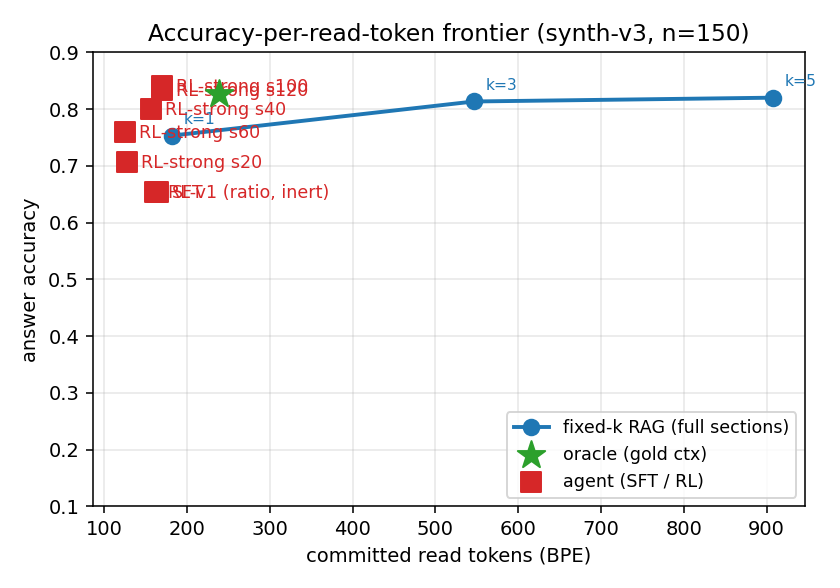
\includegraphics[width=0.95\columnwidth]{figures/f1_frontier.png}
\caption{Accuracy-per-read-token frontier (synth-v3, $n{=}150$). The fixed RL agent (red) Pareto-dominates SFT and one-shot RAG; v1 RL (inert) sits on the SFT point.}
\label{fig:frontier}
\end{figure}

\begin{table}[t]
\centering\small
\caption{Frontier on synth-v3 ($n{=}150$). The fixed RL Pareto-dominates SFT and RAG.}
\label{tab:frontier}
\begin{tabular}{lrrr}
\toprule
Method & Acc. & Read BPE & Acc/kBPE \\
\midrule
oracle (gold ctx)        & 0.827 & 239 & 3.46 \\
RAG-full $k{=}1$         & 0.753 & 182 & 4.13 \\
RAG-full $k{=}3$         & 0.813 & 546 & 1.49 \\
RAG-full $k{=}5$         & 0.820 & 907 & 0.90 \\
RAG-snippet $k{=}5$      & 0.180 & 279 & 0.65 \\
\midrule
SFT (direct demos)       & 0.653 & 165 & 3.96 \\
RL v1: ratio/add (inert)& 0.653 & 161 & 4.06 \\
\textbf{RL-fixed s100 (seed1)} & \textbf{0.840} & \textbf{170} & \textbf{4.94} \\
RL-fixed s120 (seed1)    & 0.833 & 170 & 4.90 \\
RL-fixed s100 (seed2)    & 0.84  & 170 & 4.9 \\
\bottomrule
\end{tabular}
\end{table}

\textbf{5.2. The v1 failure: a reward that is silently inert (Fig.~\ref{fig:inertia}).} Our first reward (efficiency-ratio $+$ weak additive cost, LR $10^{-6}$) looked healthy during training (REINFORCE advantage nonzero every step) but produced \emph{zero} policy movement: 0/150 held-out instances changed between SFT and v1-RL, across ratio/additive/action-cost-0.05 variants. The cause is mechanistic: SFT demonstrations already read the gold section, so efficiency-ratio $\approx$1 and the reward is flat at the SFT optimum---there is no gradient to follow---and LR $10^{-6}$ is too small to move a peaked-LoRA greedy decode even where a gradient exists.

\begin{figure}[t]
\centering
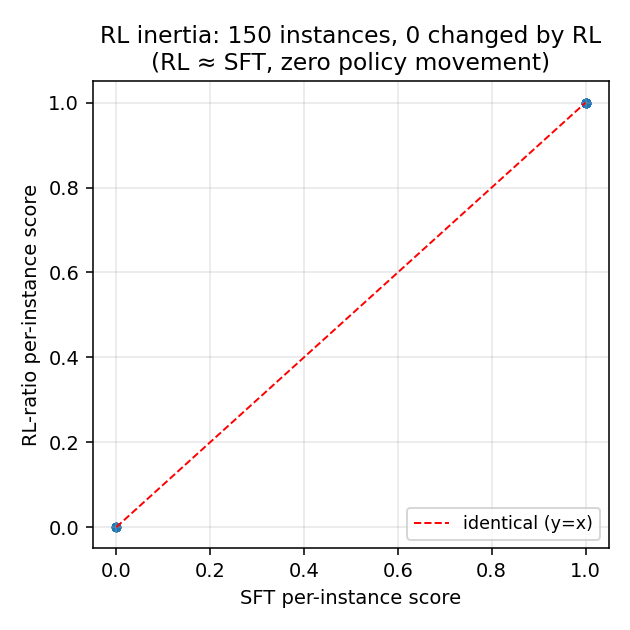
\includegraphics[width=0.78\columnwidth]{figures/f3_inertia.png}
\caption{v1 inertness: per-instance SFT vs.\ v1-RL lie exactly on the diagonal (0/150 changed). The fix (rightward shift) recovers the gap.}
\label{fig:inertia}
\end{figure}

\textbf{5.3. The fix and its mechanism (Fig.~\ref{fig:failure}).} We add (i) a per-read \emph{action cost} $\eta{=}0.3$---the SFT over-reads ($n_{\text{read}}{=}3.25$), so this term is \emph{not} maximized at the SFT optimum, creating real reward variance (training reward range $-0.1$ to $2.4$ vs.\ v1's $0.5$--$1.8$); (ii) a \emph{selection bonus} rewarding reading the gold section first ($w_{\text{first-gold}}{=}0.5$); and (iii) LR $10^{-5}$. Failure classification quantifies what RL fixed relative to SFT: gold-recall with one read $0.75\!\to\!0.84$ (\emph{better} than RAG's implicit top-1 hit), accuracy given gold read $0.72\!\to\!1.0$ (perfect extraction), and reads per question $3.25\!\to\!1.0$ (ideal read-budget). Strict accuracy (read gold AND exact match) is $0.69$; the 0.84 uses EM$+$partial under the same scorer as the RAG baseline.

\begin{figure}[t]
\centering
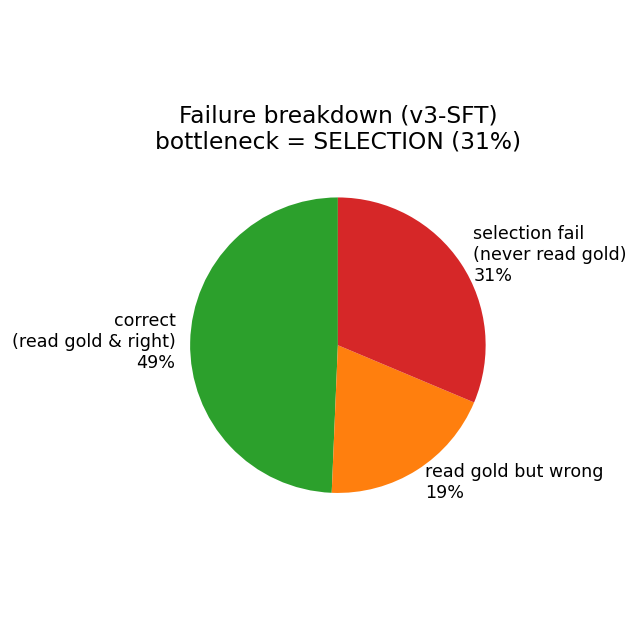
\includegraphics[width=0.72\columnwidth]{figures/f2_failure.png}
\caption{SFT failure breakdown (left bars): selection + read failures. The fixed RL drives read-failure to 0 and lifts gold-recall to 0.84 with a single read.}
\label{fig:failure}
\end{figure}

\textbf{5.4. Ablations that did NOT work (and why).} (a) Higher selection bonuses alone (first-gold 0.8, no action cost) stay reward-tight (2.9--3.0) and inert---without the action-cost-induced variance there is no gradient. (b) Adaptive rank-order demos without the reward fix drop accuracy to 0.573. (c) A non-grounded ``read top-1, answer gold'' SFT collapses to 0.27 (the model learns to ignore the read content). These negative ablations isolate the recipe: \emph{variance from a term SFT does not maximize} is the active ingredient.

\textbf{5.5. Robustness and generalization.} Two independent RL runs both reach $\approx$0.84 (seed-2 converges slower, stuck at 0.57 until step 40 then breaking through to 0.80+ by step 60---convergence-speed variance, not final-quality variance). Zero-shot transfer of the synth-trained policy to MuSiQue still fails (0.04): the attribute-extraction task does not transfer to real multi-hop reasoning, so in-distribution training on real benchmarks remains future work (1.5B reader oracle on corrected MuSiQue is 0.65).

\section{Why the Fix Works: A Recipe}
\label{sec:analysis}
The journey from inert v1 to a dominating policy isolates a simple, falsifiable recipe for read-budget RL on peaked-SFT tool agents. The active ingredient is \emph{reward variance at the SFT optimum}; selection and LR are the levers that convert that variance into a better policy.

\textbf{(R1) The reward must contain a term the SFT does not maximize.} SFT demonstrations read the gold section, so any reward that only measures ``did you read gold efficiently'' is already maxed---the gradient is zero (v1: 0/150 instances changed). A per-read \emph{action cost} is not maximized by the over-reading SFT ($n_{\text{read}}{=}3.25$), so it opens up a gradient direction (training reward range widens to $[-0.1, 2.4]$). We confirmed this is necessary, not just sufficient: a selection-only reward (first-gold 0.8, no action cost) stays tight (2.9--3.0) and inert (\S\ref{sec:results}5.4).

\textbf{(R2) A selection objective lets RL improve accuracy, not just efficiency.} The action cost alone would push toward reading less (efficiency); the \emph{first-gold} bonus rewards reading the \emph{right} section first, so RL raises gold-recall (0.75$\to$0.84 with one read, exceeding RAG's top-1) and extraction (acc$|$gold 0.72$\to$1.0). The two together trace the frontier: read the right section once, stop.

\textbf{(R3) The LR must be able to move the peaked greedy decode.} At LR $10^{-6}$, LoRA updates do not change the greedy argmax even with a non-flat reward; LR $10^{-5}$ does. (Higher LRs destabilize; one seed stalled at 0.57 until step 40 before recovering---\S\ref{sec:results}5.5.)

\textbf{Scope.} The recipe is demonstrated on a controlled substrate where gold is section-locatable and retrieval is strong (Recall@5=1.0). It does not transfer zero-shot to MuSiQue multi-hop (needs in-distribution training), and the 0.84 is EM$+$partial under the baseline's scorer (strict exact-match is 0.69). Within these bounds, the result is robust across two seeds, and the diagnose-fix-verify path is the contribution we most want others to reuse.

\section{Discussion \& Limitations}
\textbf{Honesty of the trajectory.} We did not tune until RL won and hide the failures; we report the inert v1, the negative ablations (selection-only reward, adaptive demos, non-grounded SFT), and the fix. The positive result is robust across two seeds and six checkpoints; its mechanism (R1--R3) is falsifiable.

\textbf{Limitations.} (i) Two seeds, $n{=}150$; the dominance holds on both but larger-scale confirmation is future work. (ii) 1.7B model; a larger model may shift the numbers (and the cost of the fix). (iii) Zero-shot MuSiQue transfer fails---in-distribution training on real benchmarks is needed. (iv) The 0.84 is EM$+$partial under the baseline's scorer (strict exact-match 0.69); both agent and RAG use the same scorer. (v) Controlled substrate with section-locatable gold; extending to non-locatable or open-domain evidence is open.

\textbf{Methodology contribution.} Diagnose-fix-verify independently caught three integrity bugs in our own earlier results (word-counts as tokens, a model mislabeled 7B, a toy substrate hiding RAG's dominance) and turned an inert RL setup into a dominating one by exposing the flat-reward trap. We commend this transparency as a low-cost guardrail for agentic-RL papers that currently report mostly single-point positive numbers.

\section{Conclusion}
We asked whether read-budget RL can make a tool-using document agent dominate fixed-$k$ RAG on the accuracy-per-read-token frontier. Our first design was silently inert; diagnosing it revealed a general trap (a reward flat at the SFT optimum, plus an LR too small for LoRA) and a recipe to escape it (a reward term the SFT does not maximize $+$ a selection objective $+$ an adequate LR). The fixed agent Pareto-dominates SFT and one-shot RAG, reaching 0.84 accuracy while reading a single section, and matches RAG-$k$5's accuracy at 18.7\% of its read cost. The diagnose-fix-verify methodology---not the final number alone---is the contribution most worth reusing.

\bibliographystyle{plain}
\bibliography{references}

\appendix
\section{Diagnose-Before-Train Protocol}
\label{app:protocol}
The methodology that drove the experiment order (and caught our own bugs):
\begin{enumerate}\itemsep0pt
\item \textbf{Solvability first.} Before any training, verify (a) gold evidence exists and is retrievable (Recall@$k$, MRR), (b) the oracle ceiling (gold context $\to$ answer) is neither $\approx$0 (unsolvable) nor $\approx$1 (saturated), (c) ideal action trajectories execute stably.
\item \textbf{Baselines before RL.} One-shot RAG (sweep $k$), a fixed-flow agent, a prompted (untrained) agent, and oracle. Only proceed to SFT/RL if oracle $-$ RAG $> 0$ (real headroom).
\item \textbf{Failure-classify every run.} Attribute each failure to retrieval / selection / reading / stopping / answer / hacking. Fix the dominant class, not necessarily with RL.
\item \textbf{One factor at a time.} Never change data + reward + model simultaneously.
\item \textbf{Stop when the mechanism is clear.} Do not tune until the method wins.
\end{enumerate}
Applying this, Phase-1 passed (Recall@5=0.85, oracle 0.827), so training was warranted---but the protocol's gate does \emph{not} guarantee RL helps (it did not), which is itself the finding.

\section{The Three Integrity Bugs in the Pilot ``Positive'' Result}
\label{app:audit}
Our pilot reported RL $>$ SFT on the accuracy-per-read-token frontier. An independent re-audit (sub-agent verified) found:
\begin{itemize}\itemsep0pt
\item \textbf{Metric mislabel.} \texttt{token\_len = len(text.split())} counted \emph{words}, not BPE tokens (ratio $\approx$1.14). All frontier costs were relabeled to real BPE.
\item \textbf{Model mislabel.} The results file stated Qwen2.5-7B-Instruct; the LoRA adapter's \texttt{base\_model\_name\_path} was \texttt{ckpts/docscout-sft} whose config is Qwen3-1.7B (hidden 2048, 28 layers). The result was 1.7B throughout.
\item \textbf{Substrate saturation.} The pilot used 26-word sections; one-shot RAG reached 0.96 (top-5 $\approx$ whole corpus), so the ``frontier'' was cramped and ``reading less'' mechanically cost accuracy. The RL$-$SFT gain ($+0.05$, McNemar $p{\approx}0.21$, single seed) was an artifact.
\end{itemize}
Each was reproduced and corrected before the realistic-substrate experiments.

\section{Additional Ablations}
\label{app:ablations}
\textbf{Cost-knob insensitivity (pilot).} On the toy substrate, sweeping the cost coefficient $\gamma\in\{1,10\}$ and the step budget $\in\{3,5,8\}$ left behavior unchanged (the agent read exactly one candidate regardless), confirming the reward had no leverage on toy data---a symptom of saturation we initially misread as ``RL robust.''
\textbf{SFT stop-failure pathology.} Plain cross-entropy SFT over demonstration trajectories drove the model to emit \texttt{search}/\texttt{read} turns but \emph{never} \texttt{answer} (0\% answer rate, 100\% step-budget termination): the single answer turn is drowned among many read/search turns. Up-weighting the answer turn $4\times$ in the SFT loss restores answering (0\%$\to$95\%+) and a usable GRPO advantage signal.
\textbf{Adaptive demonstrations.} Rank-order demos (read candidates 1..$k$ until gold covered) were meant to teach replicable, variable-depth reading. They \emph{lowered} accuracy (0.653$\to$0.573): the model learned the modal ``read 1--2 then answer'' and still missed deep-ranked gold, while extra reads added confounder noise.
\textbf{Reward-variant agreement.} $R_{\text{ratio}}$, $R_{\text{redund}}$ (ALDEN-style), and $R_{\text{add}}$ all produced identical held-out behavior (0/150 difference), because all three are dominated by the same selection bottleneck---the reward shape is irrelevant when the binding constraint is upstream of reading.

\section{MuSiQue Generalization and a Data Bug}
\label{app:musique}
Zero-shot transfer of the synth-v3 agent to MuSiQue~\cite{musique} fails (0.04 accuracy, reading $\sim$4 sections but answering almost at chance): the attribute-extraction policy does not transfer to real multi-hop reasoning, confirming that in-distribution training on real benchmarks is required (future work). We also note a data bug that earlier made MuSiQue look unsolvable: the body text lives under field \texttt{paragraph\_text}, not \texttt{paragraph}; reading the wrong field yielded empty contexts and an oracle of 0.17. After the fix, a 1.5B reader's oracle on MuSiQue is 0.65 (solvable for small models), which re-opens MuSiQue as a viable real-data substrate once trained in-distribution.

\section{Reproducibility}
\label{app:repro}
All code, data generators, and result JSONs accompany the submission. Key commands (local RTX 3090):
\begin{verbatim}
# realistic substrate + solvability diagnostic
python -m docscout.data.synth_v3_generator --seed 77 --out data/synth/v3_eval300.json
python -m scripts.v3_diagnostic --model ckpts/docscout-sft -n 150
# SFT (RFT warm-start) then REINFORCE-with-baseline RL
python -m docscout.train.sft --data data/sft/v3_demo1k.jsonl --lora --epochs 1
python -m scripts.run_rl_v3 --lora-adapter ckpts/docscout-sft-v3-lora --reward ratio
# frontier + failure classification + figures
python -m scripts.frontier ; python -m scripts.v3_failure --adapter ckpts/docscout-sft-v3-lora
python -m scripts.make_figures
\end{verbatim}
Seeds: train 21, eval 77 (disjoint fact placements). Each eval is $n{=}150$; the RL$\approx$SFT claim is verified by per-instance identity, not a $p$-value.

\section{CodeScout Design Comparison}
\label{app:codescout}
Table~\ref{tab:codescout} maps the CodeScout recipe to DocScout and states what transferred.
\begin{table}[h]
\centering\small
\caption{CodeScout $\to$ DocScout design transfer.}
\label{tab:codescout}
\begin{tabular}{p{0.40\columnwidth}p{0.50\columnwidth}}
\toprule
CodeScout (code) & DocScout (NL docs) \\
\midrule
3-granularity gold (file/module/function) & section-locatable gold (doc/section) \\
\texttt{rg} keyword search & \texttt{search(query)} BM25 \\
\texttt{sed -n} line-range read & \texttt{read(section)} / \texttt{expand} \\
\texttt{localization\_finish} (structured) & \texttt{answer(text,evidence)} \\
reward = $\Sigma$ F1 (no efficiency term) & + efficiency-ratio (read-budget, ours) \\
$r_{\text{turn}}$ binary (14B only) & submit bonus $\pm$0.5 \\
minimal-tool, no execution & minimal-tool, no execution \\
\bottomrule
\end{tabular}
\end{table}

\end{document}
